\documentclass{article}

\usepackage{ctex}
\usepackage[top=0.7in,bottom=0.7in,left=0.5in,right=0.5in]{geometry}
\usepackage{array}
\usepackage{multirow}
\usepackage{graphicx}
\usepackage{subfigure}
\usepackage{fancyhdr}
\usepackage{lastpage}
\usepackage{extramarks}
\usepackage{amsmath}
\usepackage{listings}
\usepackage{fontspec}
\newfontfamily\consolas{Consolas}
\usepackage{xcolor} % 定制颜色
\definecolor{mygreen}{rgb}{0,0.6,0}
\definecolor{mygray}{rgb}{0.5,0.5,0.5}
\definecolor{mymauve}{rgb}{0.58,0,0.82}
\lstset{ %
backgroundcolor=\color{white},      % choose the background color
basicstyle=\footnotesize\ttfamily,  % size of fonts used for the code
columns=fullflexible,
tabsize=4,
breaklines=true,               % automatic line breaking only at whitespace
captionpos=b,                  % sets the caption-position to bottom
commentstyle=\color{mygreen},  % comment style
escapeinside={\%*}{*)},        % if you want to add LaTeX within your code
keywordstyle=\color{blue},     % keyword style
stringstyle=\color{mymauve}\ttfamily,  % string literal style
frame=single,
rulesepcolor=\color{red!20!green!20!blue!20},
% identifierstyle=\color{red},
language=c++,
}

\newcommand{\hmwkTitle}{求有向无环图最长路径\ 实验报告}
\newcommand{\hmwkClass}{数据结构}
\newcommand{\hmwkClassInstructor}{}
\newcommand{\hmwkAuthorName}{毛子恒\ 李臻\ 张梓靖}

\pagestyle{fancy}
\lhead{\hmwkAuthorName}
\chead{\hmwkClass\ : \hmwkTitle}
\rhead{\firstxmark}
\lfoot{\lastxmark}
\cfoot{\thepage}
\renewcommand\headrulewidth{0.4pt}
\renewcommand\footrulewidth{0.4pt}

\title{\hmwkClass\ :\hmwkTitle}
\author{\hmwkAuthorName}

\setcounter{tocdepth}{1}

\begin{document}

\maketitle

\section*{小组成员}

\setlength{\tabcolsep}{9mm}
{
    \begin{table}[htbp]
        \centering
        \begin{tabular}{llll}
            班级:2019211309 & 姓名:毛子恒 & 学号:2019211397 & 分工:代码\ 文档   \\

            班级:2019211310 & 姓名:李臻   & 学号:2019211458 & 分工:测试\ 文档   \\

            班级:2019211308 & 姓名:张梓靖 & 学号:2019211379 & 分工:文档 \\
        \end{tabular}
    \end{table}
}

\tableofcontents
\newpage

\section{需求分析}

\subsection{题目描述}

给定一个有向无环图,找到图中距离最远的两个结点。

\subsection{输入描述}

程序从标准输入中读入数据。

输入的第一行包含两个整数$n,m$,用空格分隔,分别表示有向无环图的点数和边数。

接下来的$m$行,每行三个整数,用空格分隔,分别表示每个弧的弧尾、弧头和权值,顶点编号$x$的范围满足$1\leq x\leq n$,权值为正整数。

\subsection{输出描述}

程序向标准输出中输出结果。

输出分为以下四种情况:

\begin{enumerate}
    \item 输入合法,程序正常运行结束,此时输出一行三个整数,用空格分隔,分别表示最长的距离和这两个顶点的编号。
    \item 输入的有向无环图没有边或者结点数少于2,此时程序输出一个字符串“No solution.”表示无解。
    \item 输入的弧头、弧尾或者权值信息范围有误,或者此图不是有向无环图,此时程序输出一个字符串“Invalid input.”。
    \item 程序发生运行时错误,比如内存分配失败等,此时程序没有输出。
\end{enumerate}

\subsection{样例输入输出}

\subsubsection{样例输入输出1}

【输入】

\begin{lstlisting}[
    basicstyle=\small\consolas]
4 4
3 4 34
1 3 24
2 4 56
2 3 11
\end{lstlisting}

【输出】

\begin{lstlisting}[
    basicstyle=\small\consolas]
58 1 4
\end{lstlisting}

\subsubsection{样例输入输出2}

【输入】(samples/sample2.in)

\begin{lstlisting}[
    basicstyle=\small\consolas]
50 75
15 18 10
28 36 64
29 45 22
24 49 66
3 35 48
31 48 15
14 29 20
48 49 60
40 42 80
42 50 40
2 23 10
1 48 98
21 28 86
5 27 99
21 26 30
17 28 46
24 50 34
15 31 100
13 37 47
32 33 74
25 34 12
8 29 60
20 37 93
25 50 5
26 31 18
26 35 26
34 45 92
26 44 51
10 20 70
25 28 85
26 46 58
28 39 51
23 35 66
23 43 45
35 43 76
7 45 76
33 41 58
21 42 44
36 37 86
23 41 51
44 50 37
4 12 60
26 30 29
26 39 20
6 30 15
35 47 91
32 34 32
7 34 46
17 25 14
41 45 82
25 27 92
10 17 11
20 48 7
32 46 56
8 49 31
12 32 23
42 48 87
35 41 19
35 49 6
25 47 46
38 42 60
46 50 50
2 41 96
29 47 59
9 20 1
26 27 15
2 25 93
34 46 81
40 45 31
27 49 67
39 50 53
12 19 11
43 48 15
38 40 54
45 49 26
\end{lstlisting}

【输出】

\begin{lstlisting}[
    basicstyle=\small\consolas]
328 2 37
\end{lstlisting}

\subsubsection{样例输入输出3}

【输入】

\begin{lstlisting}[
    basicstyle=\small\consolas]
5 0
\end{lstlisting}

【输出】

\begin{lstlisting}[
    basicstyle=\small\consolas]
No solution.
\end{lstlisting}

\subsubsection{样例输入输出4}

【输入】

\begin{lstlisting}[
    basicstyle=\small\consolas]
2 3
8 2 12 
1 2 3
1 2 7
\end{lstlisting}

【输出】

\begin{lstlisting}[
    basicstyle=\small\consolas]
Invalid input.
\end{lstlisting}

\subsection{程序功能}

程序找到图中距离最大的两个点并且输出这两个点及其距离。

\section{概要设计}

\subsection{问题解决的思路}

程序建立采用邻接表存储的图,先求出拓扑序,再求出以每个点为源点到其余顶点的距离及其路径,记录所有情况中离源点的最大距离以及对应的源点。

\subsection{图的设计}

\begin{lstlisting}[language={C},
    numbers=left,
    numberstyle=\tiny\consolas,
    basicstyle=\small\consolas]
// 数据对象
typedef struct edge
{
    int v, val;
    struct edge * next;
} Edge;

extern int n, m; // n为点数,m为边数
extern int * ind; // 各个顶点的入度
extern int * dist; // 以各个顶点为终点的的最长距离
extern int * start; // 距离这个点最远的点的编号
extern Edge ** firstEdge;

/*
 * 操作:初始化有向无环图
 * 后件:初始化firstEdge、ind、dist、start数组
 */
void initGraph();

/*
 * 操作:向图中加入弧
 * 前件:u,v是弧尾、弧头的编号,val是弧的权值
 * 后件:图中加入这条边
 */
void addEdge(int u, int v, int val);

/*
 * 操作:有向无环图的拓扑排序,求出dist和start数组的值
 * 前件:firstEdge中存储有向无环图的信息
 * 后件:如果有向无环图合法,则返回0,并且dist中存储源点至各个点的最短距离,start中记录最远的点的编号;否则函数返回1
 */
bool topologicalSort();

/*
 * 操作:释放有向无环图的空间
 * 后件:释放各条边的空间,以及firstEdge、ind、dist、start数组的空间
 */
void destroyGraph();

\end{lstlisting}

\subsection{主程序的流程}

\begin{enumerate}
    \item 输入,建图
    \item 拓扑排序求以每个点为终点的最长距离
    \item 比较最长距离,找到图中的最长路径
    \item 输出
    \item 释放有向无环图的空间
\end{enumerate}

\subsection{各程序模块之间的层次关系}

程序模块层次关系图如图1。

\begin{figure}[htbp]

    \centering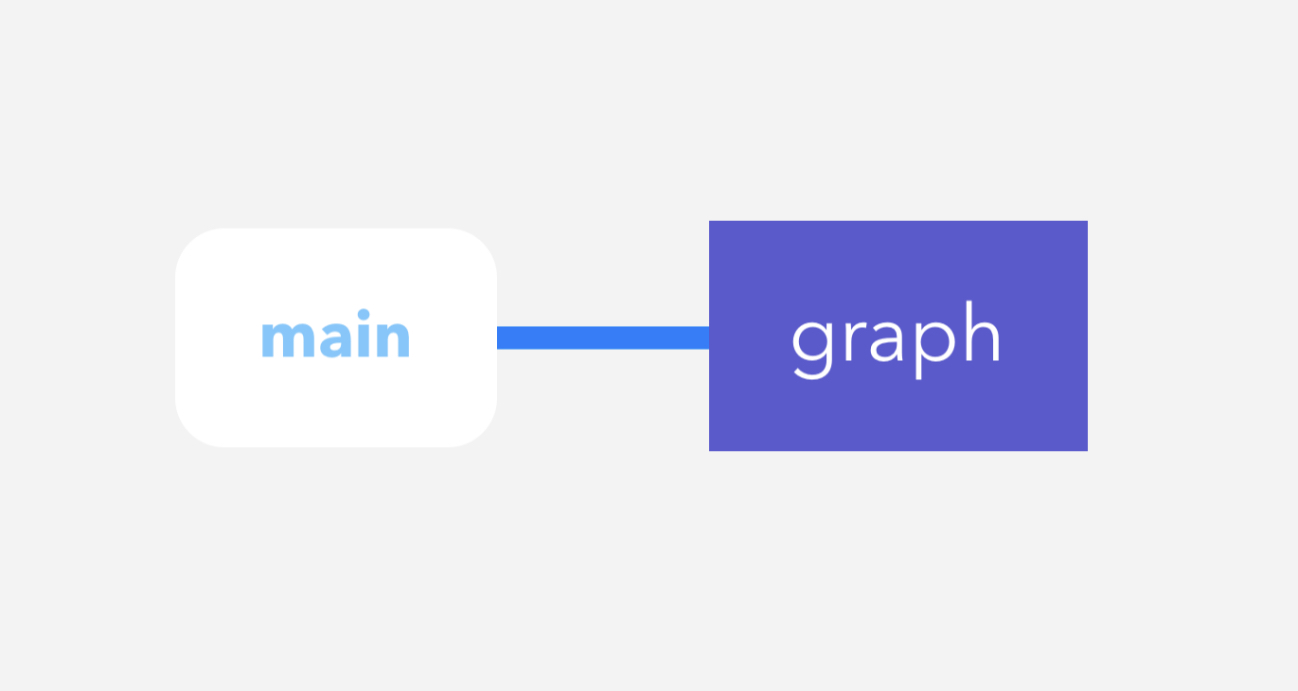
\includegraphics[width=0.4\textwidth]{./Images/pic5_1.png}

    \caption{程序模块层次关系}

\end{figure}

\section{详细设计}

\subsection{图的实现}

图的设计中基本操作的伪代码算法如下:

\begin{lstlisting}[language={C},
    numbers=left,
    numberstyle=\tiny\consolas,
    basicstyle=\small\consolas]
// 初始化有向无环图
void initGraph()
{
    初始化firstEdge、ind、dist、start数组并分配内存
    if (内存分配失败)
        异常退出
}

// 向图中加入边
void addEdge(int u, int v, int val)
{
    初始化新的边元素temp
    if (内存分配失败)
        异常退出
    temp->val <- val
    temp->v <- v
    temp->next <- firstEdge[u]
    firstEdge[u] <- temp
    v的入度+1
}

// 有向无环图的拓扑排序
bool topologicalSort()
{
    定义临时数组tempdist用于临时存放每个源点到各个顶点的距离,order为拓扑序(同时是队列)
    if (内存分配失败)
        异常退出
    遍历所有顶点,将入度为0的点入队
    while (队列不为空)
    {
        u 为队首元素
        遍历以u为弧尾的每一条弧
        {
            弧头的入度-1
            if (弧头的入度为0)
                弧头入队
        }
    }
    遍历每个顶点,通过检查入度判断这个图是不是有向无环图,不是则返回-1
    for (i = 1 to n)
    {
        初始化tempdist数组为极大值
        设置起点order[i]的tempdist为0
        for (j = i to n)
        {
            u <- order[j]
            if (tempdist[u]不为极大值 并且 tempdist[u] > dist[u])
            {
                dist[u] <- tempdist[u]
                start[u] <- order[u]
            }
            遍历以u为弧尾的每一条弧
                if (tempdist[u] + 边权 > tempdist[弧头])
                    tempdist[弧头] = tempdist[u] + 边权
        }
    }
    释放空间
}

// 释放有向无环图的空间
void destroyGraph()
{
    释放有向无环图各边元素的空间,以及firstEdge、ind、dist、start数组的空间
}
\end{lstlisting}

\subsection{函数的调用关系图}

函数调用关系图如图2。

\begin{figure}[htbp]

    \centering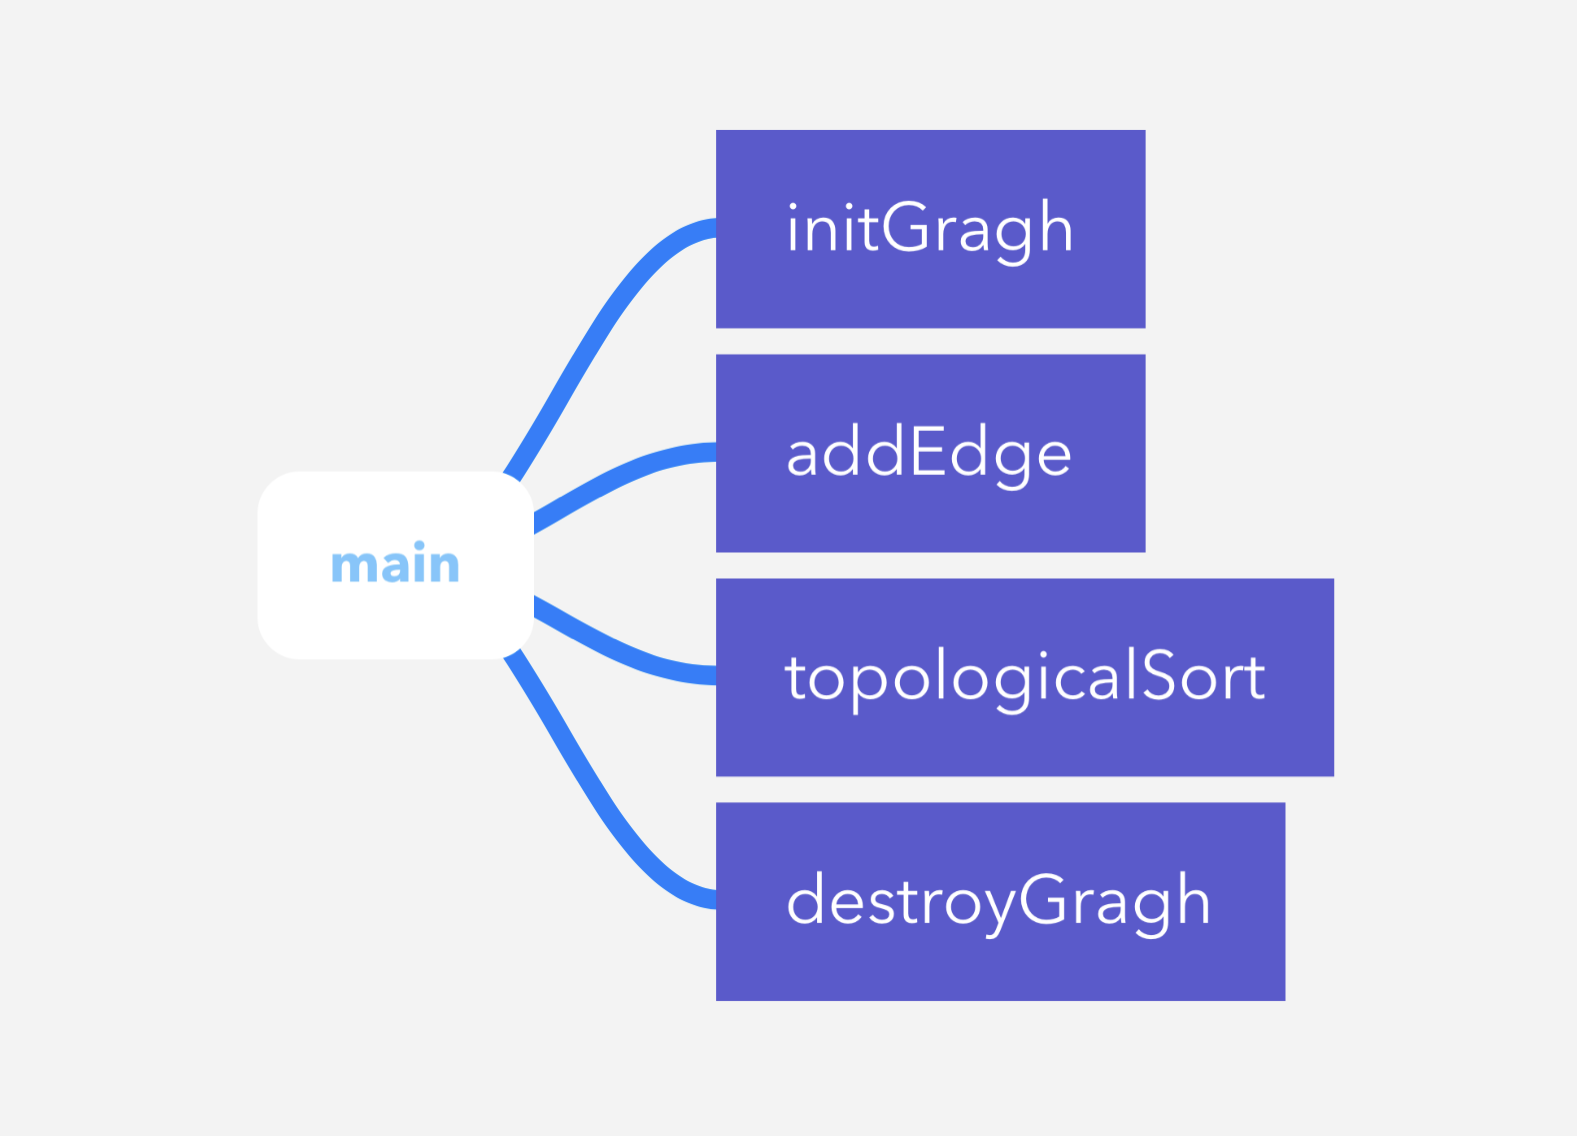
\includegraphics[width=0.4\textwidth]{./Images/pic5_2.png}

    \caption{函数调用关系图}

\end{figure}

\section{调试分析报告}

\subsection{调试过程中遇到的问题和思考}

初步设计算法时从一个虚拟源点起求出到各个顶点的距离,在这其中找到最大值,但是不符合题意,之后改成了以每个点为起点分别求距离,再在这其中找最大值。

\subsection{设计实现的回顾讨论}

通过一次处理出拓扑序,免去了之后求距离时每次再求一遍拓扑序,提高了效率。

本题中不采用深度优先遍历的方式求拓扑排序的原因,其一是编程复杂度较高,涉及传参等问题,其二是这种方法无法检测图的合法性。

\subsection{算法复杂度分析}

initgraph,addEdge函数的复杂度为$O(1)$。

topologicalSort函数的复杂度为$O(n(n+m))$

destroyGraph函数的复杂度为$O(e)$

主函数的时间复杂度为$O(n+m)$,整体时间复杂度为$O(n(n+m))$。

整体空间复杂度为$O(n+e)$

可以发现当图较为稀疏时相比floyd算法,本算法的时间复杂度优势较大,但是当图十分稠密时,由于邻接表本身常数的限制,可能运行时间和floyd算法接近。

\subsection{改进设想的经验和体会}

\subsubsection{改进1}

在更新tempdist的过程中可以发现有些时候肯定产生不了更优的解,一部分情况可以跳过。

比如,某些节点的tempdist[u]已经比dist[u]小,这个时候这个结点的部分后继的tempdist就可以跳过不需要再计算了,因为产生不了更长的距离。

\subsubsection{改进2}

可以去除重边。应当有常数级别的优化。

\section{用户使用说明}

使用gcc编译生成可执行文件。

\begin{lstlisting}[language={bash},
    basicstyle=\small\consolas]
gcc -o main -std=c11 main.c graph.c
\end{lstlisting}

执行可执行文件:

\begin{lstlisting}[language={bash},
    basicstyle=\small\consolas]
./main
\end{lstlisting}

在Windows cmd下:

\begin{lstlisting}[language={bash},
    basicstyle=\small\consolas]
main
\end{lstlisting}

之后通过标准输入输入数据,格式参考1.2节,程序通过标准输出输出结果。如果输入合法并且程序正常运行结束,主函数返回值为0。

\section{测试结果}

测试环节分为三个步骤。

\subsection{测试第一部分}

对1.4节给出的样例进行测试。

\subsection{测试第二部分}

测试边界条件。

【输入】

\begin{lstlisting}[
    basicstyle=\small\consolas]
2 2
1 2 3
2 1 2
\end{lstlisting}

【输出】

\begin{lstlisting}[
    basicstyle=\small\consolas]
Invalid input.
\end{lstlisting}

【输入】

\begin{lstlisting}[
    basicstyle=\small\consolas]
3 2
1 2 3
2 3 -1
\end{lstlisting}

【输出】

\begin{lstlisting}[
    basicstyle=\small\consolas]
Invalid input.
\end{lstlisting}

【输入】(samples/sample7.in)

(一个规模较大的样例,略)

【输出】

\begin{lstlisting}[
    basicstyle=\small\consolas]
767 2 974
\end{lstlisting}

\subsection{测试第三部分}

测试在macOS\ Big\ Sur\ 11.0.1下进行。

在$n,m<=10$,$n,m<=100$,$n<=1000,m<=1500$的范围下分别随机生成1000组测试数据,分别输入到本算法和另外实现的floyd算法(testing/floyd.cpp)中计算,比较其输出。

3000组数据中输出均相同。

数据生成程序(testing/data.cpp)如下:

\begin{lstlisting}[language={C++},
    numbers=left,
    numberstyle=\tiny\consolas,
    basicstyle=\small\consolas]
#include <bits/stdc++.h>
using namespace std;

int main(int argc, char *argv[])
{
    srand(time(0));
    int n = atoi(argv[1]), m = atoi(argv[2]);
    printf("%d %d\n", n, m);
    for (int i = 1; i <= m; ++i)
    {
        int x = rand() % (n - 1) + 1;
        printf("%d %d %d\n", x, rand() % (n - x) + x + 1, rand() % 100 + 1);
    }
    return 0;
}
\end{lstlisting}

传入两个参数,分别是$n,m$的大小。

比对脚本(testing/chk.sh)如下:

\begin{lstlisting}[language={bash},
    numbers=left,
    numberstyle=\tiny\consolas,
    basicstyle=\small\consolas]
for i in {1..100}
do
    sleep 1
    ./data 1000 1500 >in.in
    ./main <in.in >out.out
    ./floyd <in.in >outt.out
    if ! diff out.out outt.out
    then
        break
    fi
    echo "Correct"
done
\end{lstlisting}

\end{document}